\section{Presentazione}
Per lo sviluppo di questo sito si è deciso di puntare ad un'estetica semplice e intuitiva, trasportando l'utente con colori che ricordino i fiori e la natura: sono state usate sfumature delicate e che ricordano la natura e molto rilassanti per l'occhio. Il sito è stato sviluppato secondo questa idea anche nella sua parte admin.\\Per facilitare gli sviluppatori del sito, si è deciso di inserire nei fogli di stile delle variabili per i colori, in modo tale che qualora ci fosse bisogno di cambiare il colore in una qualche parte del sito, risulta molto più facile. Ogni variabile rappresenta o una porzione di sito o una precisa funzionalità (per esempio mostrare un messaggio di errore).\\\\Per lo sviluppo del sito, si è usata la tecnica del \textit{Responsive Web Design}, in modo tale da ottimizzare la visualizzazione del sito (sia \textit{lato cliente} che \textit{lato admin}) per qualsiasi tipo di dispositivo. 

\subsection{Desktop}
Il layout desktop presenta una disposizione a tutta pagina in maniera orizzontale dei contenuti. Si è deciso comunque di rendere l'interfaccia pulita e di non accavallare più contenuti in poco spazio. 
\subsubsection{Cliente}
Nella parte \textit{cliente}, il sito presenta un menù di navigazione orizzontale fisso, con lo sfondo leggermente trasparente per renderlo più delicato.
Si è deciso di adottare un footer corposo, con tutte le informazioni importanti (come telefono, orari di apertura, ecc...), in modo tale da lasciarle sempre visibili per il cliente che visita il sito, insieme ai vari social-media.
\begin{center}
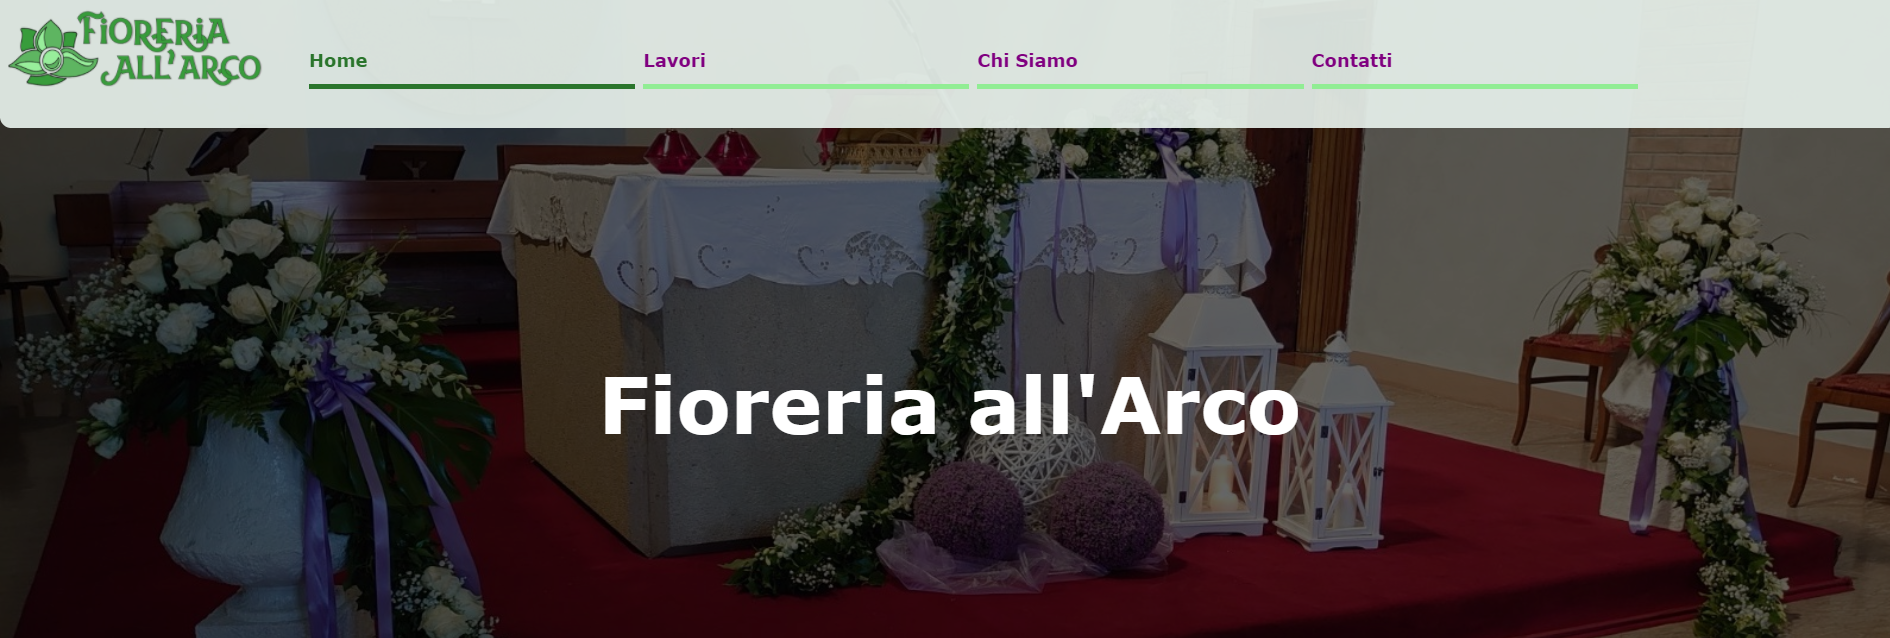
\includegraphics[scale = 0.35]{../latex/images/desktopclient.png}\\[0.5cm]
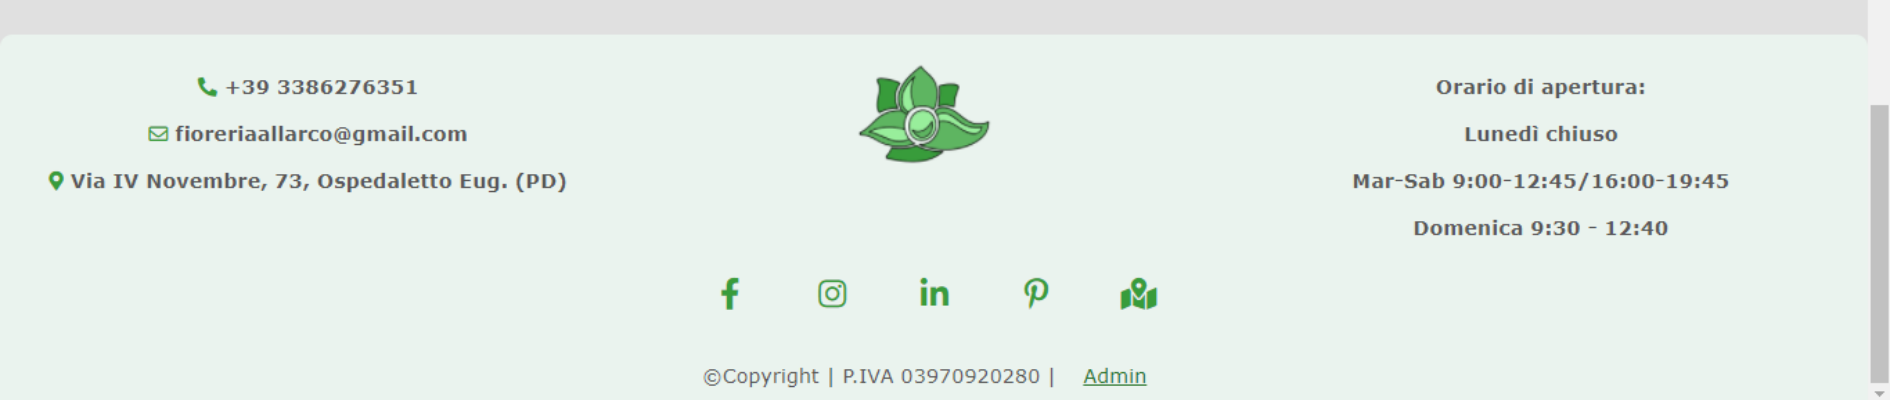
\includegraphics[scale = 0.35]{../latex/images/desktopclient-footer.png}\\[0.5cm]
\end{center}
\subsubsection{Admin}
Nella parte \textit{admin}, il sito presenta un menù di navigazione verticale fisso sulla sinistra con tutte le varie voci. L'idea era di rendere il più facile possibile la navigazione e soprattutto di avere molto spazio per la pagina di gestione delle varie modifiche.
\begin{center}
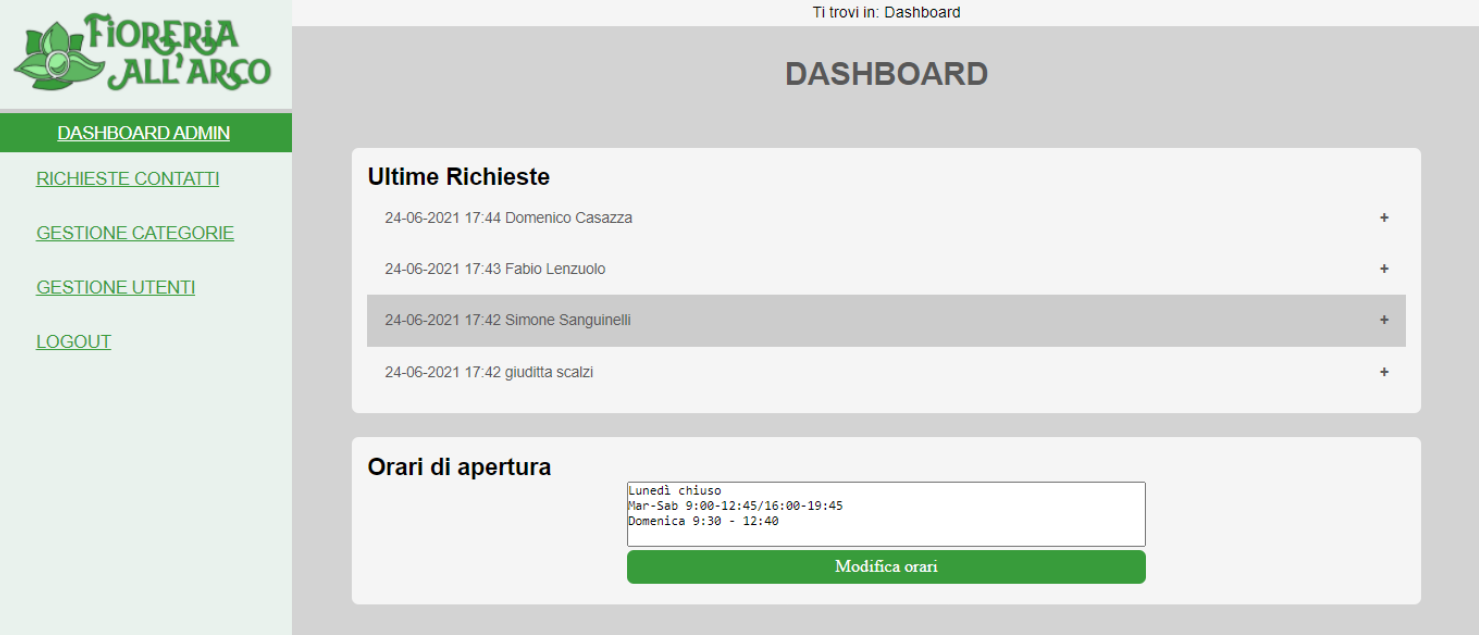
\includegraphics[scale = 0.4]{../latex/images/desktopadmin.png}\\[0.5cm]
\end{center}
\subsection{Mobile}
Il layout mobile è principalmente improntato su una disposizione verticale dei vari elementi della pagina, distanziando tra loro gli elementi cliccabili per evitare che l'user clicchi involontariamente sull'elemento sbagliato. 
\subsubsection{Cliente}
Per la parte \textit{cliente} l'header raggruppa il menù di navigazione in un menù ad hamburger, mentre il footer contiene solo gli orari di apertura e i social-media visto che le altre informazioni(email, numero di telefono e indirizzo) sono reperibili nella pagina dei Contatti. Per le pagine di esposizione dei lavori, in particolare per la gallery, si è deciso di passare da un layout a 4 immagini per riga ad un layout a 2 immagini per riga per evitare che le foto fossero troppo piccole e troppo vicine tra di loro.
\begin{center}
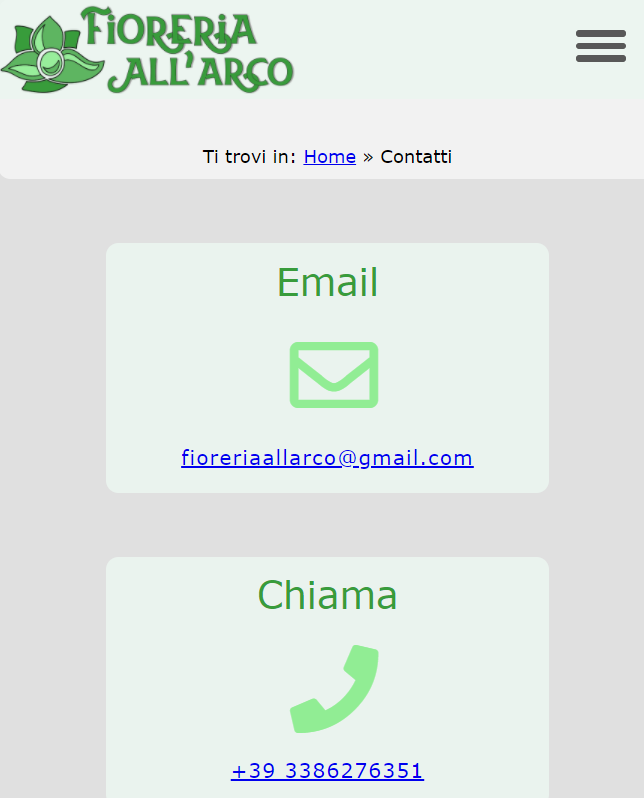
\includegraphics[scale = 0.35]{../latex/images/mobileclient.png}\\[0.5cm]
\end{center}
\subsubsection{Admin}
Per la parte \textit{admin} si è scelto di posizionare il menù di navigazione in alto e di mostrare sempre le varie voci del menù, per lo stesso ragionamento adottato nella versione desktop.
\begin{center}
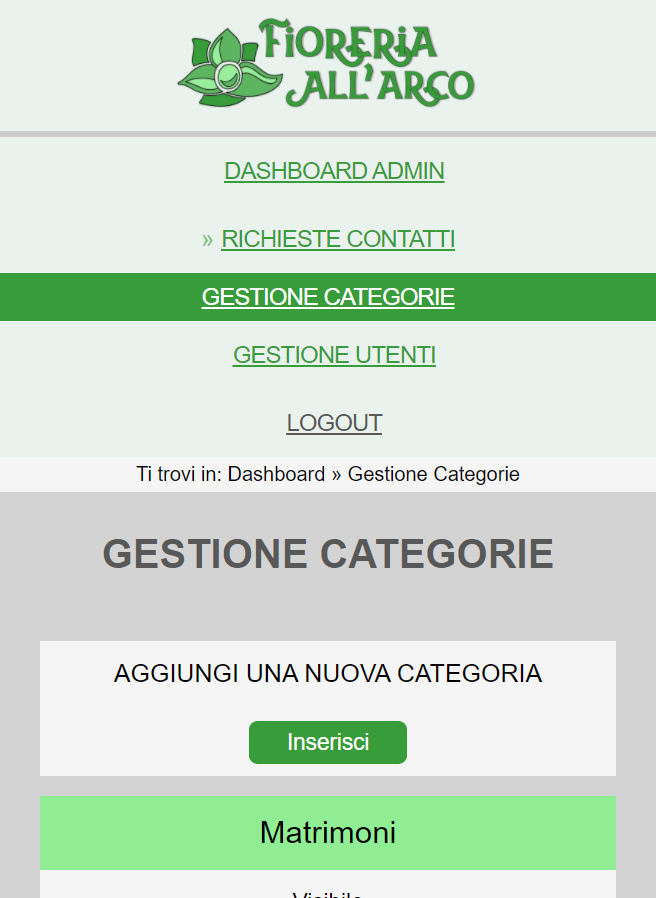
\includegraphics[scale = 0.35]{../latex/images/mobileadmin.png}\\[0.5cm]
\end{center}
\subsection{Print}
Sia per il lato \textit{cliente} che per il lato \textit{admin}, è stato creato un foglio di stile per la stampa di una pagina del sito: si è deciso quindi come formattare la pagina in vista della stampa, togliendo immagini e colori. \\Viene ora riportato uno screen della stampa di una pagina nel sito cliente e nella sezione admin.
\begin{center}
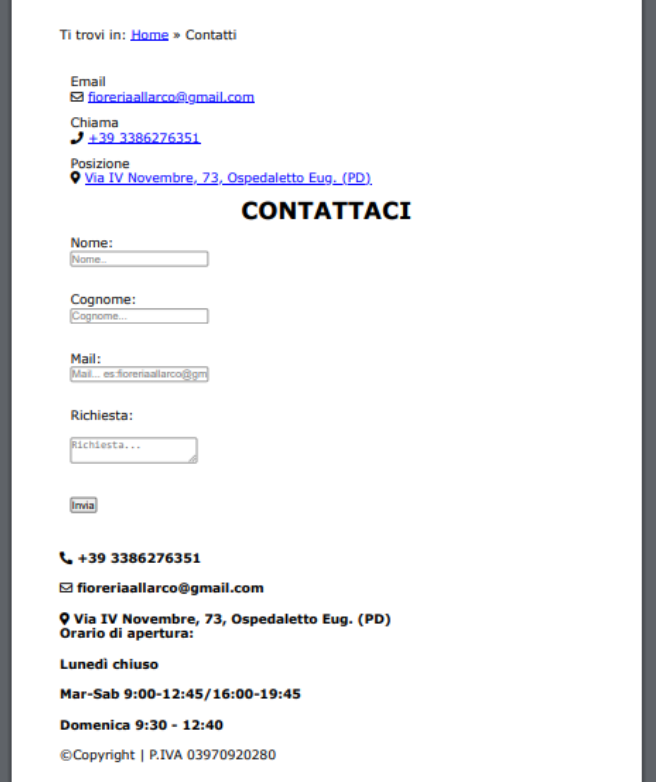
\includegraphics[width = 0.35 \textwidth]{../latex/images/clientprint.png}\hspace{5em}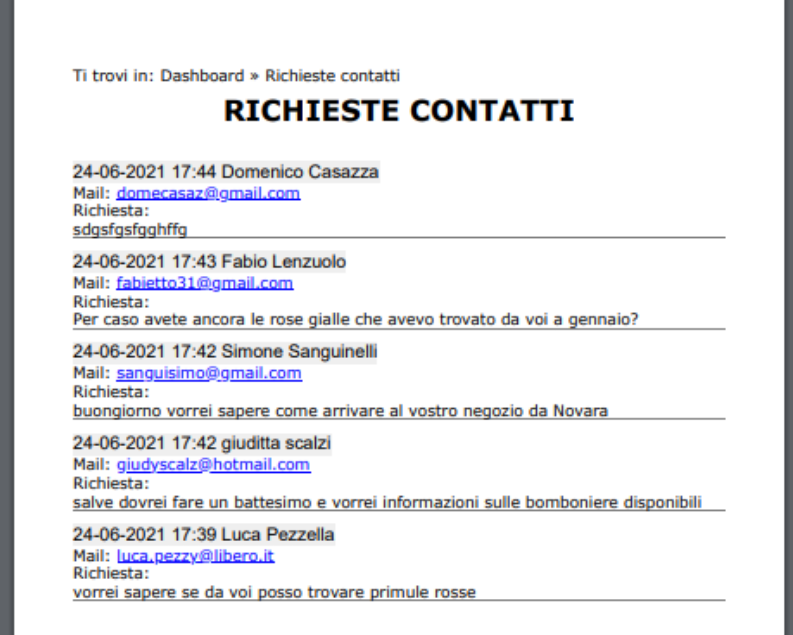
\includegraphics[width = 0.45 \textwidth]{../latex/images/adminprint.png}
\end{center}

